\paragraph{Задание 4}
\subparagraph{Условие:}
Отфильтровать в захвате IP пакеты. Определить статистические данные:

\begin{itemize}
    \item процентное соотношение трафика разных протоколов стека tcp/ip в сети;
    \item средний, минимальный, максимальный размеры пакета.
\end{itemize}

На примере любого IP-пакета указать структуры протоколов Ethernet и IP. Отметить поля заголовков и описать их и интерпретировать их значения.

\subparagraph{Решение:} \hspace{0pt}

\subparagraph{1-ый подпункт} \hspace{0pt}

В поле фильтра ввожу <<tcp>>. Жму синую кнопку со стрелкой <<Apply this filter string to the display.>>.
Результат на рисунке \textbf{\ref{fig:4-1-filter-tcp} (стр. \pageref{fig:4-1-filter-tcp})}.

Для показа процентного соотношение трафика разных протоколов стека tcp в сети
жму <<Statistics>>, затем <<Protocal Hierarchy>>.
Результат на рисунке \textbf{\ref{fig:4-1-Protocol-Hierarchy-tcp} (стр. \pageref{fig:4-1-Protocol-Hierarchy-tcp})}.

\begin{figure}[!htp]
    \centering
    \begin{minipage}{.49\textwidth}
        \centering
        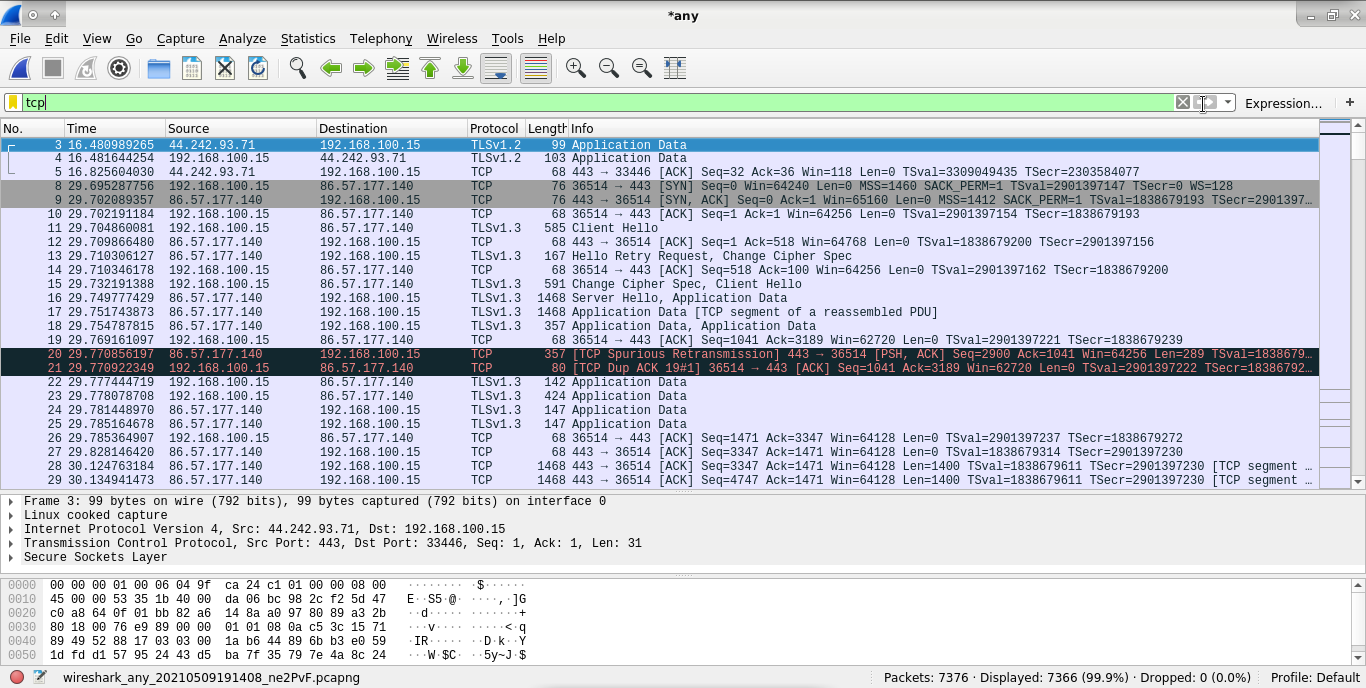
\includegraphics[width=.99\textwidth]
        {../_INCLUDES/main/task4/4-1-filter-tcp.png}
        \caption{Wireshark filter:tcp}
        \label{fig:4-1-filter-tcp}
    \end{minipage}
    \begin{minipage}{.49\textwidth}
        \centering
        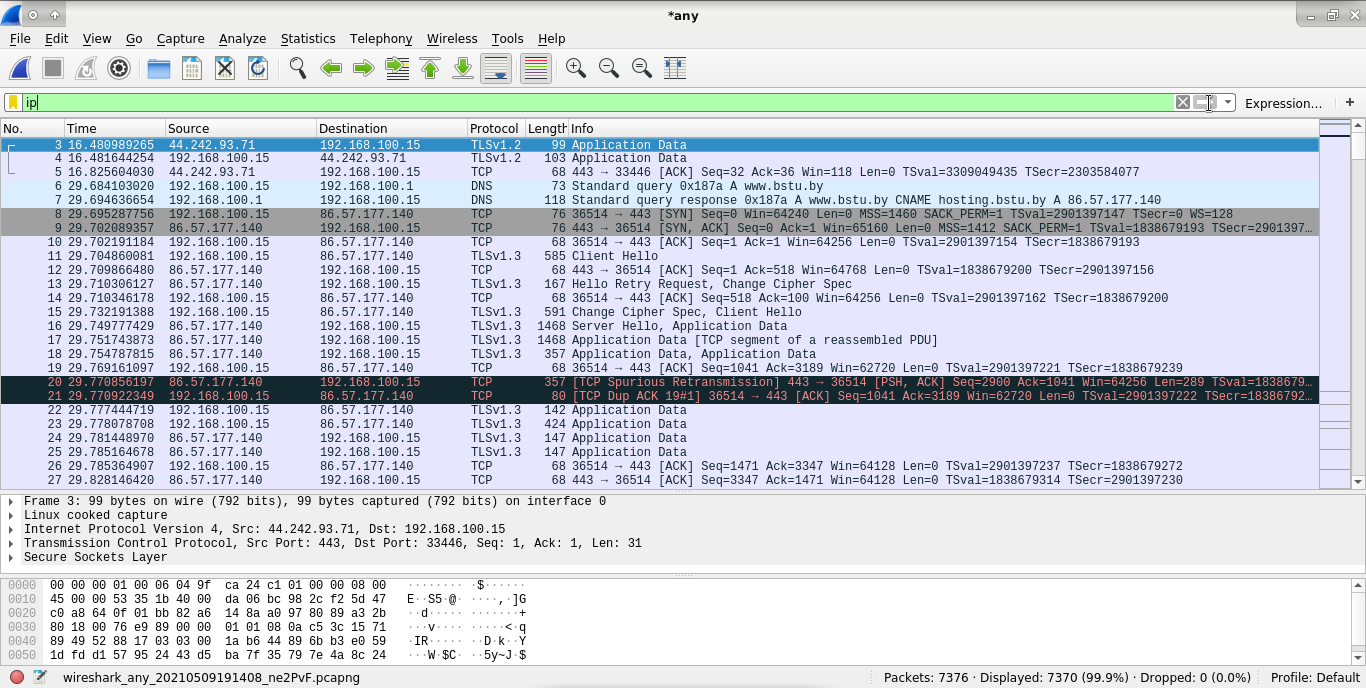
\includegraphics[width=.99\textwidth]
        {../_INCLUDES/main/task4/4-1-filter-ip.png}
        \caption{Wireshark filter:ip}
        \label{fig:4-1-filter-ip}
    \end{minipage}
\end{figure}

\begin{figure}[!htp]
    \centering
    \begin{minipage}{.49\textwidth}
        \centering
        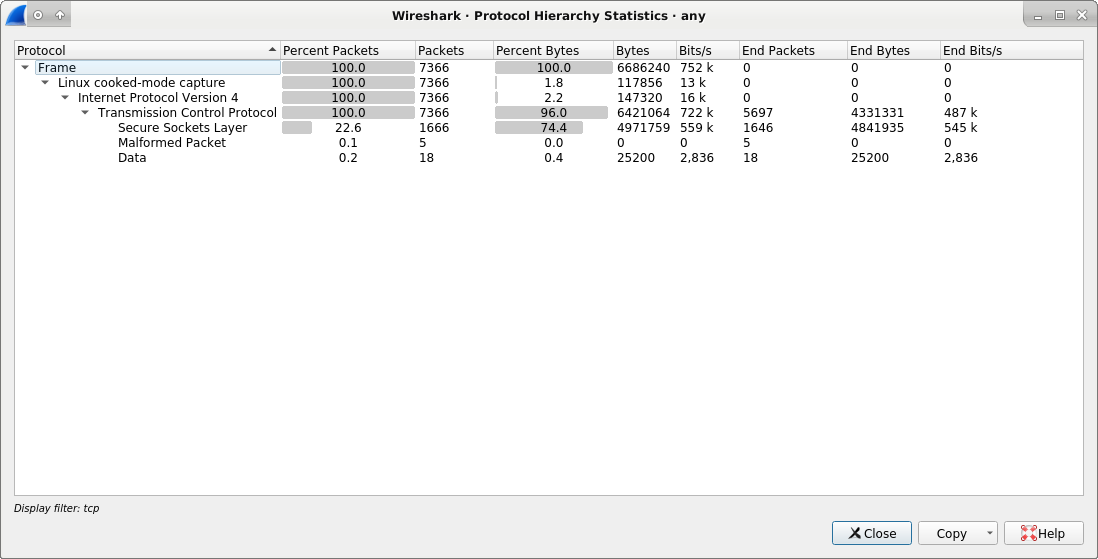
\includegraphics[width=.99\textwidth]
        {../_INCLUDES/main/task4/4-1-Protocol-Hierarchy-tcp.png}
        \caption{Protocol Hierarchy filter:tcp}
        \label{fig:4-1-Protocol-Hierarchy-tcp}
    \end{minipage}
    \begin{minipage}{.49\textwidth}
        \centering
        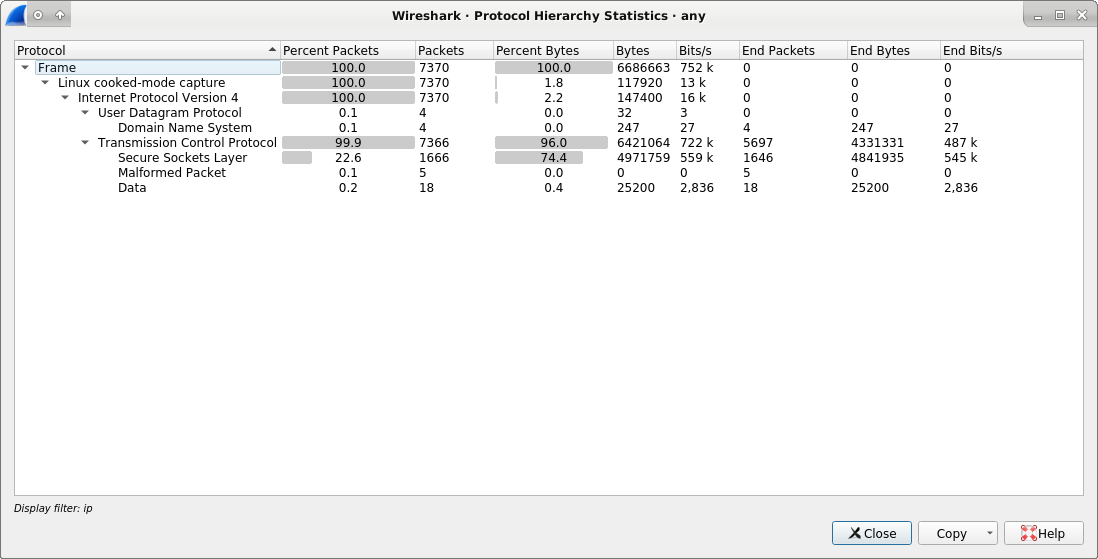
\includegraphics[width=.99\textwidth]
        {../_INCLUDES/main/task4/4-1-Protocol-Hierarchy-ip.png}
        \caption{Protocol Hierarchy filter:ip}
        \label{fig:4-1-Protocol-Hierarchy-ip}
    \end{minipage}
\end{figure}

\newpage

\subparagraph{2-ой подпункт} \hspace{0pt}

Для показа среднего, минимального, максимального размера пакета tcp
жму <<Statistics>>, затем <<Packet Lengths>>.
Результат на рисунке \textbf{\ref{fig:4-2-Packet-Length-filter-tcp} (стр. \pageref{fig:4-2-Packet-Length-filter-tcp})}.

Для показа среднего, минимального, максимального размера пакета ip
жму <<Statistics>>, затем <<Packet Lengths>>.
Результат на рисунке \textbf{\ref{fig:4-2-Packet-Length-filter-ip} (стр. \pageref{fig:4-2-Packet-Length-filter-ip})}.

\begin{figure}[!htp]
    \centering
    \begin{minipage}{.49\textwidth}
        \centering
        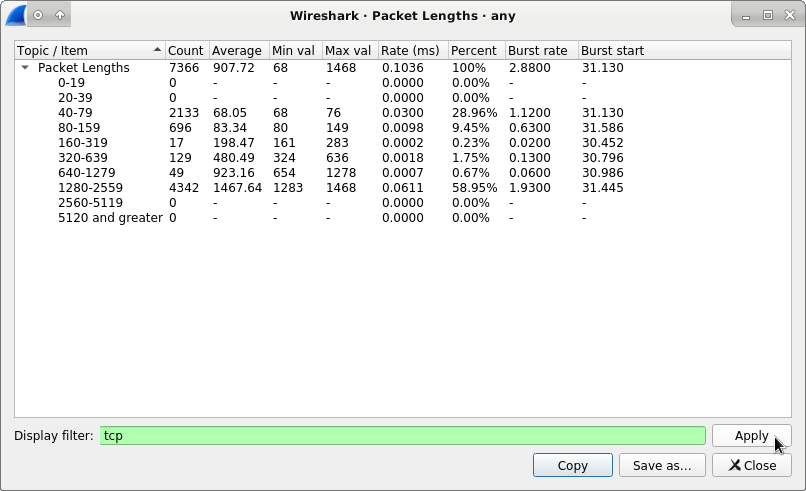
\includegraphics[width=.99\textwidth]
        {../_INCLUDES/main/task4/4-2-Packet-Length-filter-tcp.png}
        \caption{Packet Length filter:tcp}
        \label{fig:4-2-Packet-Length-filter-tcp}
    \end{minipage}
    \begin{minipage}{.49\textwidth}
        \centering
        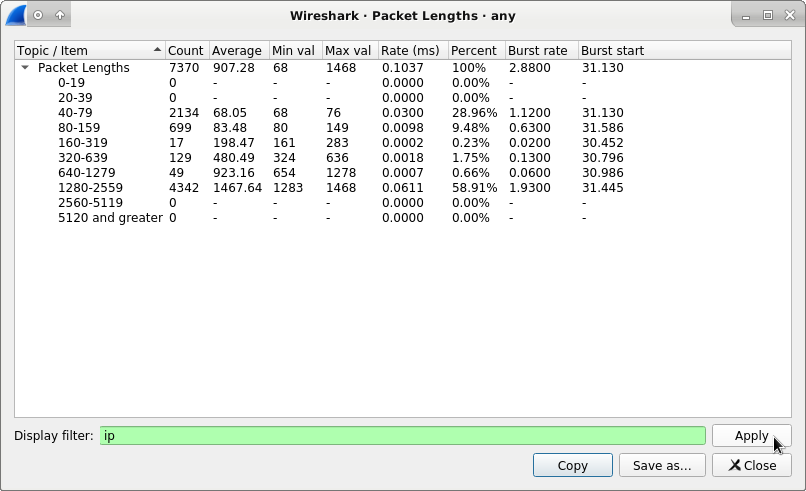
\includegraphics[width=.99\textwidth]
        {../_INCLUDES/main/task4/4-2-Packet-Length-filter-ip.png}
        \caption{Packet Length filter:ip}
        \label{fig:4-2-Packet-Length-filter-ip}
    \end{minipage}
\end{figure}

\subparagraph{После пунктное задание} \hspace{0pt}

Взяв случайный пакет жму на него.
Снизу в окне смотрю её структуру.
Результат на рисунке \textbf{\ref{fig:4-3} (стр. \pageref{fig:4-3})}.

\begin{figure}[!htp]
    \centering
    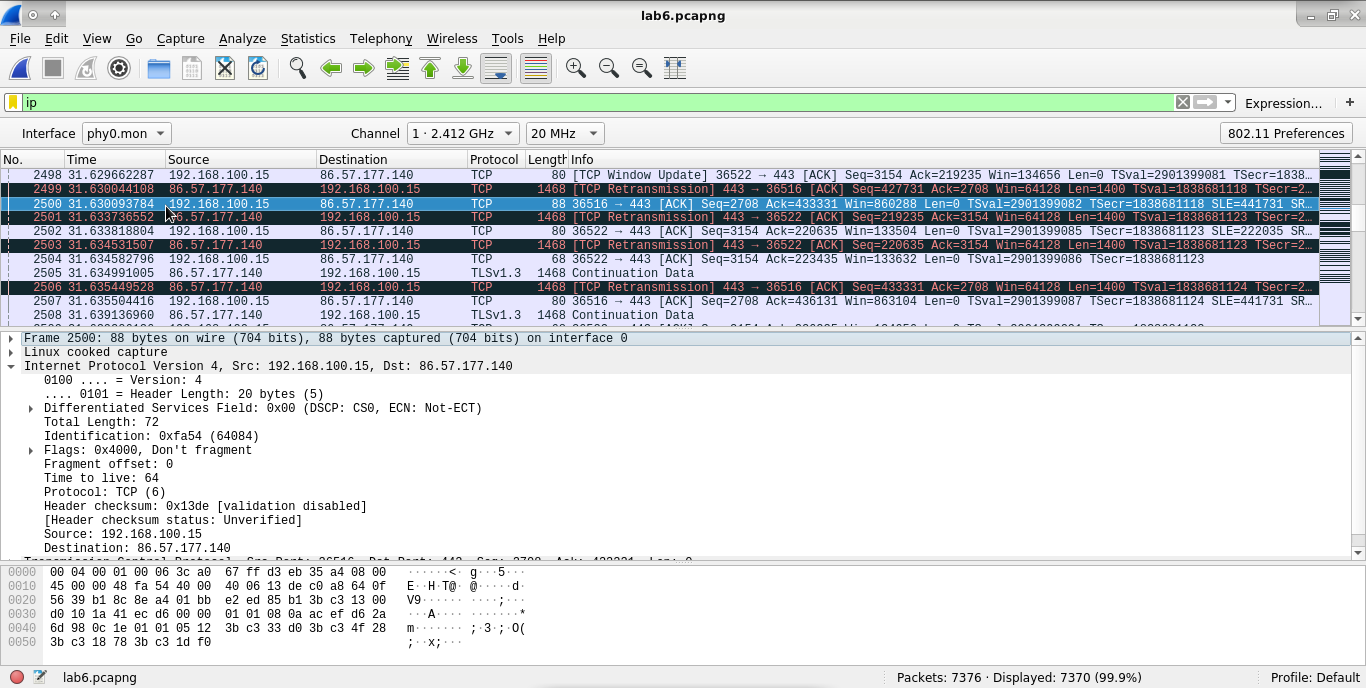
\includegraphics[width=.99\textwidth]
    {../_INCLUDES/main/task4/4-3.png}
    \caption{Структура пакета}
    \label{fig:4-3}
\end{figure}